\documentclass[11pt, a4paper]{report}
\usepackage[utf8]{inputenc}
\usepackage{calc}
\usepackage[T1]{fontenc}
\usepackage{geometry}
\usepackage{graphicx}
\usepackage{hyperref}
\usepackage{amsmath}
\usepackage{booktabs}
\usepackage{tabularx}
\usepackage{multirow}
\usepackage[sort&compress]{natbib}
\usepackage[french]{babel}
\usepackage{enumitem}

\geometry{margin=2.5cm}
\setlength{\parskip}{0.5em}

\begin{document}

\begin{titlepage}
    \centering
    \begin{figure}[h]
        \centering
        
\includegraphics[width=0.5\textwidth]{./assets/logo_polymtl.png}
        \label{fig:logo_polymtl}
    \end{figure}

    {\scshape\LARGE Polytechnique Montréal \par}
    \vspace{1cm}
    {\scshape\Large INF8245AE – Machine Learning \par}
    \vspace{4cm}
    {\huge\bfseries Assignment 1 – Linear Regression\par}
    \vspace{2cm}
    {\Large\itshape Mattéo Colavita - 2142009\par}
    \vfill
    \vspace{0.8cm}
    {\large 2025-09-26\par}
\end{titlepage}

\section{Question 1: Linear and Weighted Ridge Regression}

\begin{figure}
\centering
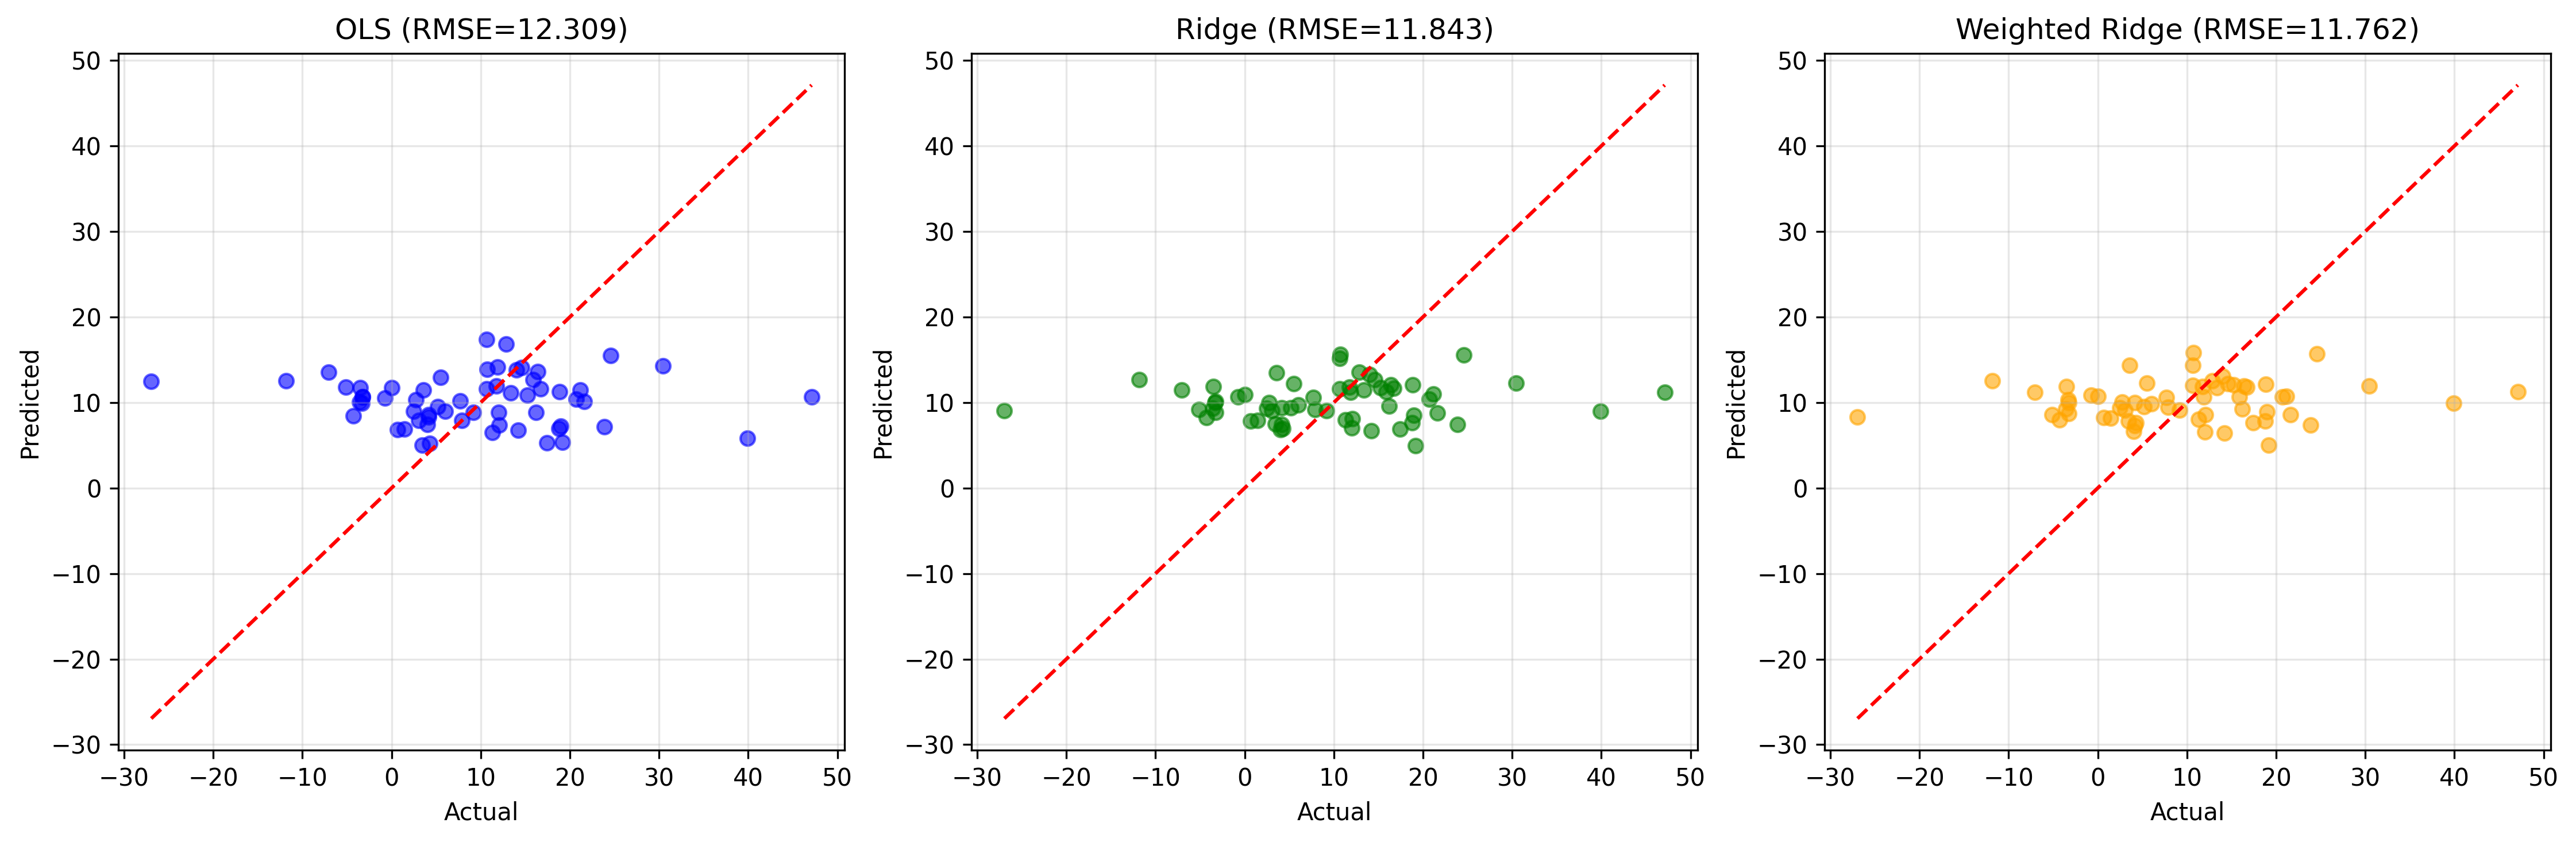
\includegraphics[width=0.8\textwidth]{./assets/regression_comparison.png}
\caption{Comparison of predictions from linear, ridge and weighted ridge regression on the test set.}
\label{fig:linear_vs_weighted_ridge}
\end{figure}

\section{Question 2: Cross-Validation}

\begin{table}[h!]
\centering
\begin{tabular}{|l|c|c|c|c|c|c|}
\hline
\textbf{Metric} & \textbf{Best $\lambda$} & \textbf{$\lambda$=0.01} & \textbf{$\lambda$=0.1} & \textbf{$\lambda$=1} & \textbf{$\lambda$=10} & \textbf{$\lambda$=100} \\
\hline
MAE & 10 & 7.381 & 7.316 & 7.140 & 7.110 & 7.817 \\
\hline
MaxError & 100 & 27.758 & 27.681 & 27.559 & 27.476 & 27.095 \\
\hline
RMSE & 10 & 9.855 & 9.772 & 9.577 & 9.532 & 10.101 \\
\hline
\end{tabular}
\caption{Mean MAE, MaxError, and RMSE scores obtained via 5-fold cross-validation for different values of $\lambda$ in ridge regression.}
\label{tab:cross_validation_results}
\end{table}

\section{Question 3: Gradient Descent for Ridge Regression}

\begin{figure}[h!]
    \centering
    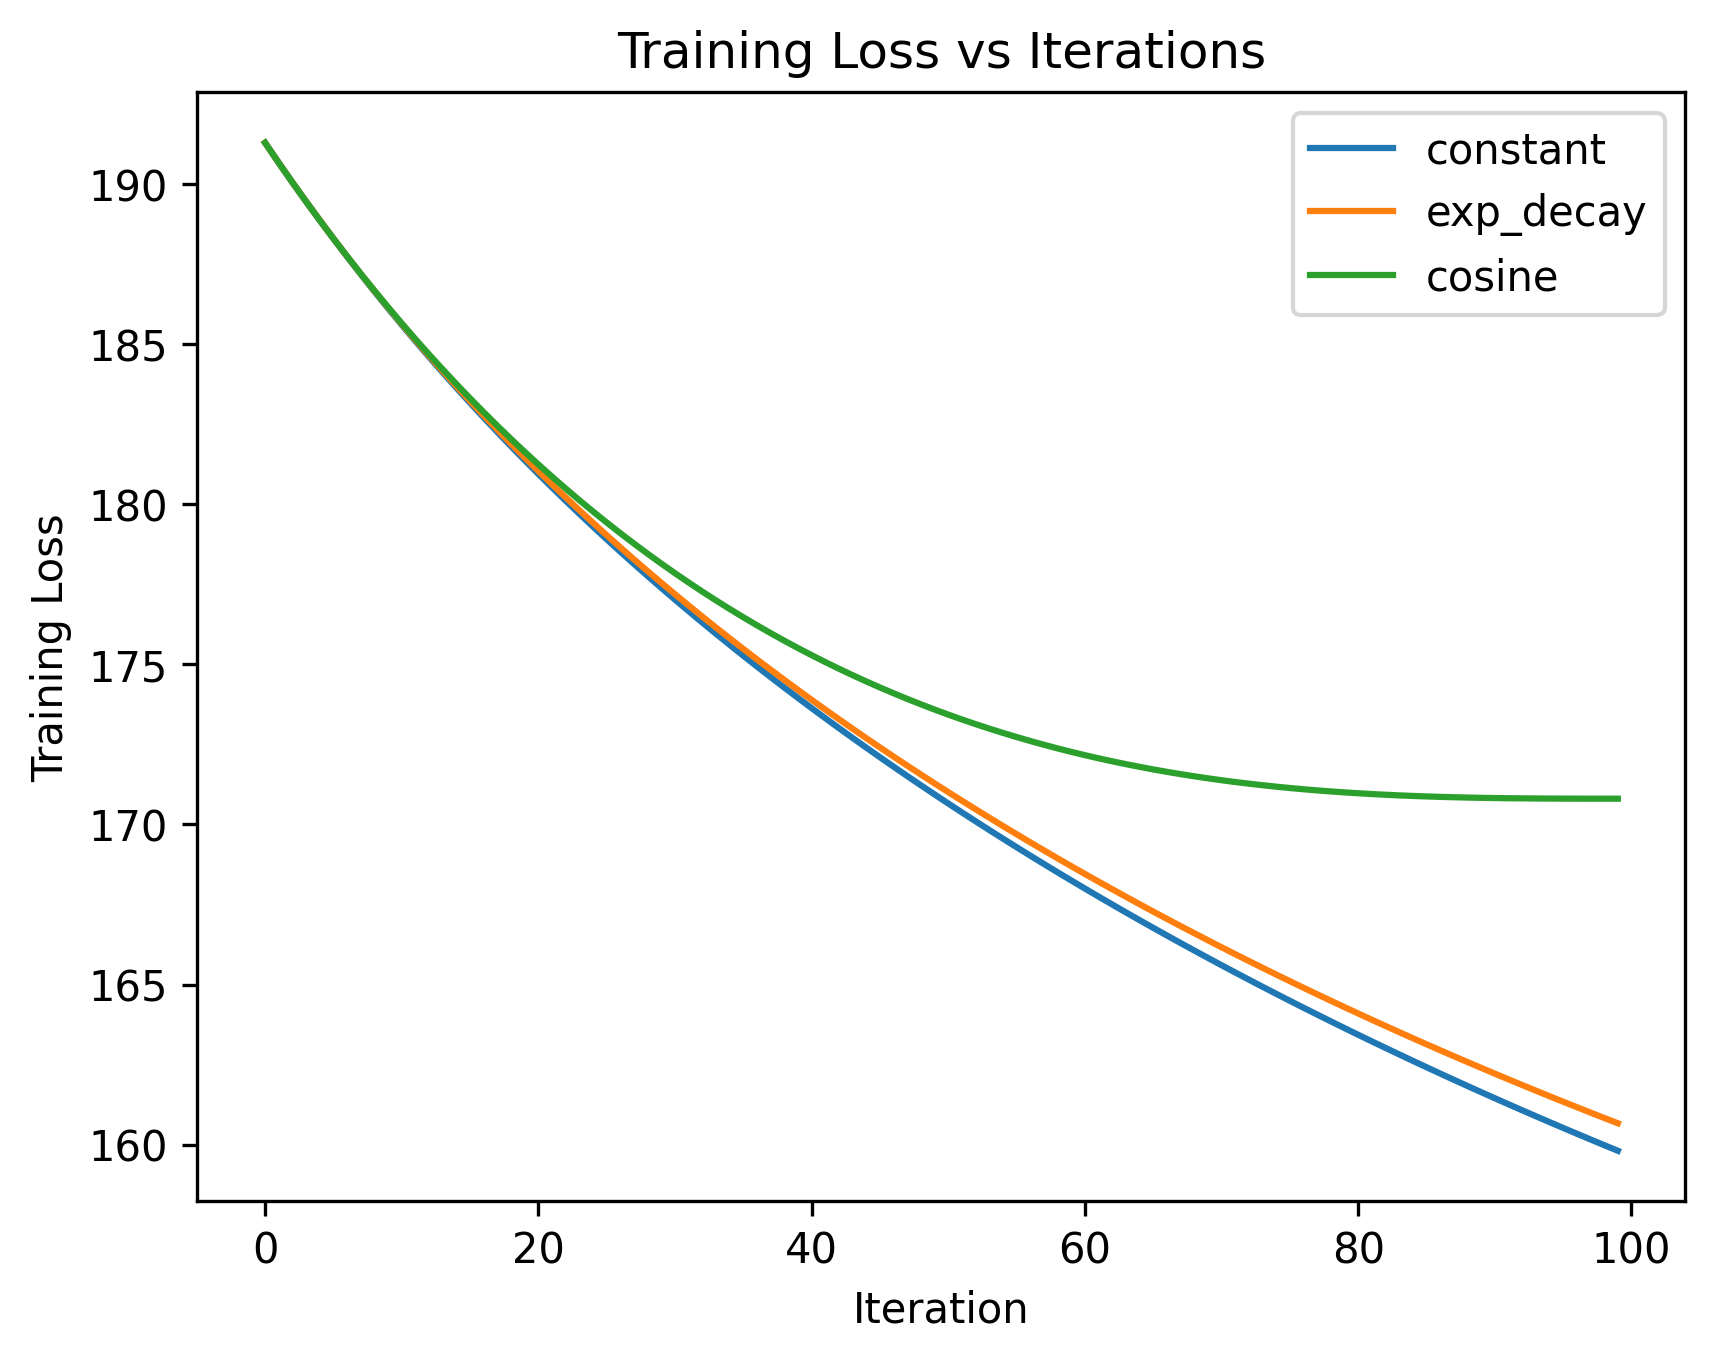
\includegraphics[width=0.8\textwidth]{./assets/training_loss_comparison.png}
    \caption{Training loss vs iterations for different learning rate schedules in gradient descent for ridge regression.}
    \label{fig:training_loss_comparison}
\end{figure}

\begin{table}[h!]
\centering
\begin{tabular}{|l|c|}
\hline
\textbf{Learning Rate Schedule} & \textbf{RMSE} \\
\hline
Constant & 13.890951849807372 \\
\hline
Exponential Decay & 13.928319736225347 \\
\hline
Cosine Annealing & 14.347341446546864 \\
\hline
\end{tabular}
\caption{RMSE results for different learning rate schedules in gradient descent for ridge regression.}
\label{tab:learning_rate_schedules}
\end{table}



\end{document}

